\recipe{Izzy's Mum's Burnt Aubergine Veggie Chilli}
\label{recipe:burnt_aubergine_veggie_chilli}
\makes{x portions}
\worktime{\SI{10} \minute}
\totaltime{\SI{10} \minute}
\source{\href{https://www.bbcgoodfood.com/}{bbc good food}}

\begin{figure}[h]
  	\centering
  	
  	\begin{tikzpicture}
  		% Save the image in a box to get its dimensions
  		\sbox0{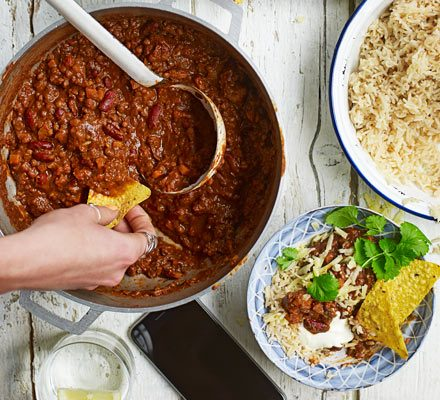
\includegraphics[width = \linewidth]{images/burnt-aubergine-chilli.jpg}}%
  
  		% Draw a clipping rectangle with rounded corners
  		\path[clip, rounded corners=0.5cm] (0,0) rectangle (\wd0,5cm);
  
  		% Place the image inside the clipped area
  		\node[inner sep=0pt, outer sep=0pt, anchor=center] at (0.5\linewidth, 2cm) {\usebox0};
	\end{tikzpicture}

\end{figure}

\begin{ingredients}

  \item 1 aubergine
  \item \SI{1}{\tablespoon} olive oil or rapeseed oil
  \item 1 red onion diced
  \item 2 carrots finely diced
  \item \SI{70}{\gram} puy lentils or green lentils, rinsed
  \item \SI{30}{\gram} red lentils rinsed
  \item \SI{400}{\gram} can kidney beans
  \item \SI{3}{\tablespoon} dark soy sauce
  \item \SI{400}{\gram} can chopped tomatoes
  \item \SI{20}{\gram} dark chocolate finely chopped
  \item \qty{0.25}{\teaspoon} chilli powder
  \item \SI{2}{\teaspoon} dried oregano
  \item \SI{2}{\teaspoon} ground cumin
  \item \SI{2}{\teaspoon} sweet smoked paprika
  \item \SI{1}{\teaspoon} coriander
  \item \SI{1}{\teaspoon} cinnamon
  \item \SI{800}{\milli \litre} vegetable stock
  \item $1/2$ lime juiced
\ingroup{To serve}
  \item brown rice
  \item tortilla chips
\end{ingredients}


\begin{method}
  	If you have a gas hob, put the aubergine directly onto a lit ring to char
completely, turning occasionally with kitchen tongs, until burnt all
over. Alternatively, use a barbecue or heat the grill to its highest setting
and cook, turning occasionally, until completely blackened (the grill
won’t give you the same smoky flavour). Set aside to cool on a plate,
then peel off the charred skin and remove the stem. Roughly chop the
flesh and set aside.

In a large pan, heat the oil, add the onion and carrots with a pinch of
salt, and fry over a low-medium heat for 15-20 mins until the carrots
have softened.

Add the aubergine, both types of lentils, the kidney beans with the
liquid from the can, soy sauce, tomatoes, chocolate, chilli powder,
oregano and the spices. Stir to combine, then pour in the stock. Bring
to the boil, then turn down the heat to very low. Cover with a lid and
cook for 1½ hrs, checking and stirring every 15-20 mins to prevent it
from burning.

Remove the lid and let the mixture simmer over a low-medium heat,
stirring occasionally, for about 15 mins until you get a thick sauce. Stir
in the lime juice and taste for seasoning – add more salt if needed.
Serve hot over rice with whichever accompaniments you want!
  
\end{method}




